% Tipo de documento
\documentclass[12pt]{article}

% Configuracion de paquetes
\usepackage[T1]{fontenc}
\usepackage[utf8]{inputenc}
\usepackage[spanish, es-tabla]{babel}
\usepackage{amsmath}
\usepackage{amssymb, amsfonts, latexsym, cancel}
\usepackage{graphicx}
\usepackage{epstopdf}
\usepackage{float}
\usepackage{subfigure}
\usepackage{array}
\usepackage{longtable}
\usepackage{bm}
\usepackage[lmargin=2cm, rmargin=2cm, top=2.5cm, bottom=2cm]{geometry}
\usepackage{fancyhdr}
\usepackage{enumerate}
\usepackage{listings}
\usepackage{multirow}

% Configuracion de pagina
\parindent=0.5cm

% Modo de inicio y pie de pagina
\pagestyle{fancy}

\fancyhead{}
\fancyhead[C]{Calentador por induccón}
\fancyhead[R]{
\includegraphics[scale=0.06]{src/institucion/Logo_uner-434x331.png}}
\renewcommand{\headrulewidth}{0.9pt}

\fancyfoot{}
\fancyfoot[R]{\thepage}
\fancyfoot[L]{Gabriel Andrés Aguirre}
\renewcommand{\footrulewidth}{0.5pt}

% Inicio del documento
\begin{document}

% Inicio de la caratula
\begin{titlepage}
\begin{center}
% Nombre de la institucion
\vspace*{2\baselineskip}
\hrule height 3pt
\vspace*{0.5\baselineskip}
{\Huge \textbf{Presentación de proyecto N$^\circ$2}}
\vspace*{0.5\baselineskip}
\hrule
% Logo de la facultad
\vspace*{10\baselineskip}

\includegraphics[scale=0.35]{src/institucion/Logo_fcal-1174x247.png}
\vspace*{2\baselineskip}
% Nombre del trabajo y tipo
\textbf{\\CALENTADOR POR INDUCCIÓN\\}
\textbf{Electrónica básica y digital}
% Nombre de los integrantes y fecha
\vfill
GABRIEL ANDRÉS AGUIRRE \\
\today
\end{center}
\end{titlepage}

% Indice
\tableofcontents
\thispagestyle{empty}
\newpage

% Desarrollo del trabajo
\setcounter{page}{1}

\section{Introducción}

\subsection{Objetivos de la materia}
El objetivo que tiene la materia es que, a travez de los conocimientos adquiridos a los largo de la asignatura, poder desarrolar un circuito de utilidad para una aplicación práctica. Para luego proceder al armado del mismo.

\subsection{Descripción del proyecto}

\subsection{Calentador por inducción magnética}
Una corriente eléctrica se genera mediante un conductor que tiene un movimiento relativo respecto a un campo magnético. Una bobina giratoria en un campo magnético induce una fuerza electromotriz alterna, la cual origina una corriente alterna. Este proceso es conocido como inducción electromagnética y es el principio de operación en el cual se basan muchos dispositivos eléctricos.

\begin{figure}[H]
\centering
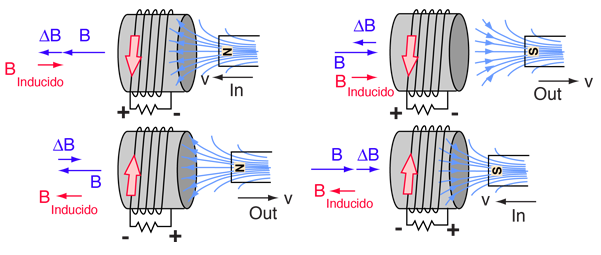
\includegraphics[scale=1.9]{src/images/Induccion.png}
\caption{Fenomeno de la inducción}
\label{fgr:Induccion}
\end{figure}

El calentamiento por inducción es un método de obtención de calor que aprovecha las perdidas en un material ferromágnetico. Este método permite que el calor sea obtenido de manera rápida y continua. El proceso de calentamiento se basa en la utilización de corrientes eléctricas que inducen un campo magnético.

El calentamiento por inducción genera calor aprovechable, continuo, rápido y no contribuye al
calentamiento global al evitar la producción de gases de efecto invernadero.

\begin{figure}[H]
\centering
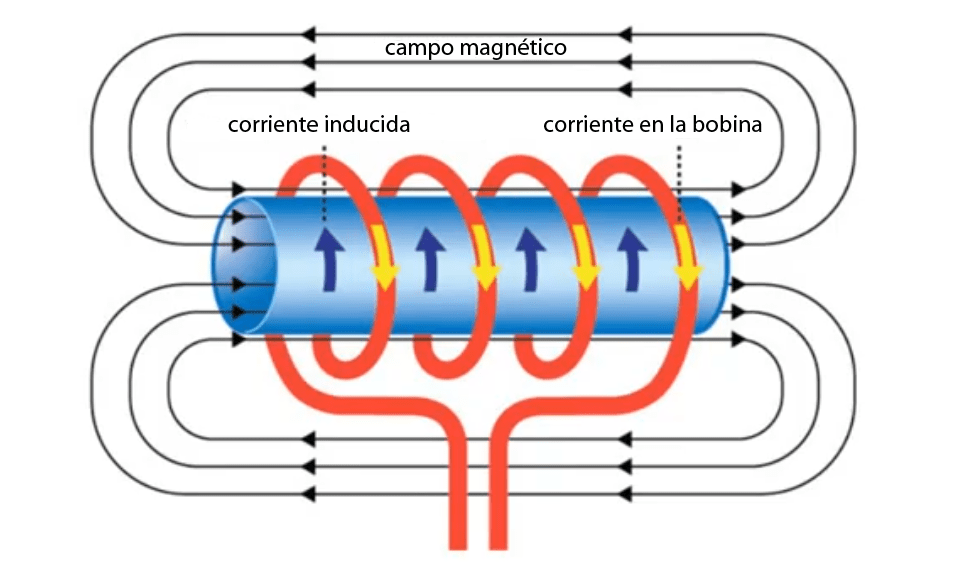
\includegraphics[scale=0.27]{src/images/Calentador_por_induccion.png}
\caption{Un tipo de calentador por inducción}
\label{fgr:Calentador_por_induccion}
\end{figure}

\subsection{Aplicaciones de un calentador por inducción magnética}
Normalmente utilizadas en cocinas que utilizan el principio por inducción, para elevar la temperatura de algún recipiente en el que se cocina un alimento o se quiere esterilizar un utencillo.

\begin{figure}[H]
\centering
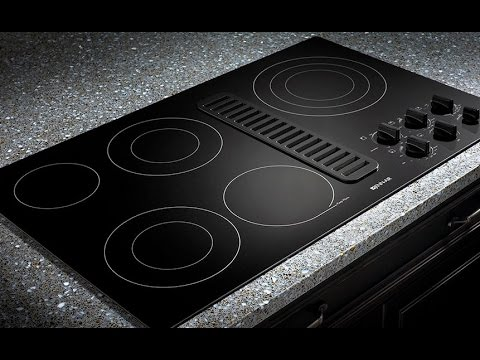
\includegraphics[scale=0.65]{src/images/Cocina.jpg}
\caption{Cocina que utiliza el principio de inducción}
\label{fgr:Cocina}
\end{figure}

Como calentadores de piezas mecánicas de gran tamaño y rapides. Comunmente se pueden ver en un industria de metalmecánica hornos de gran tamaño que en su interior yace el metal que quiere ser manipulado o transformado.

\begin{figure}[H]
\centering
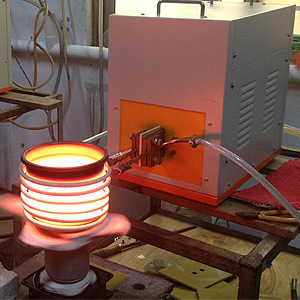
\includegraphics[scale=0.75]{src/images/Calentador_de_juntas.jpg}
\caption{Calentador de piezas industrial que utiliza el principio de inducción}
\label{fgr:Calentador_de_juntas}
\end{figure}

\section{Marco teórico}

\subsection{Conceptos físicos}

\subsection{Bobina}
Una bobina no es mas que un enrrollamiento de cable de determinada forma, que concentre el campo magnetico que cruza por el hacia una dirección determinada.

\begin{figure}[H]
\centering
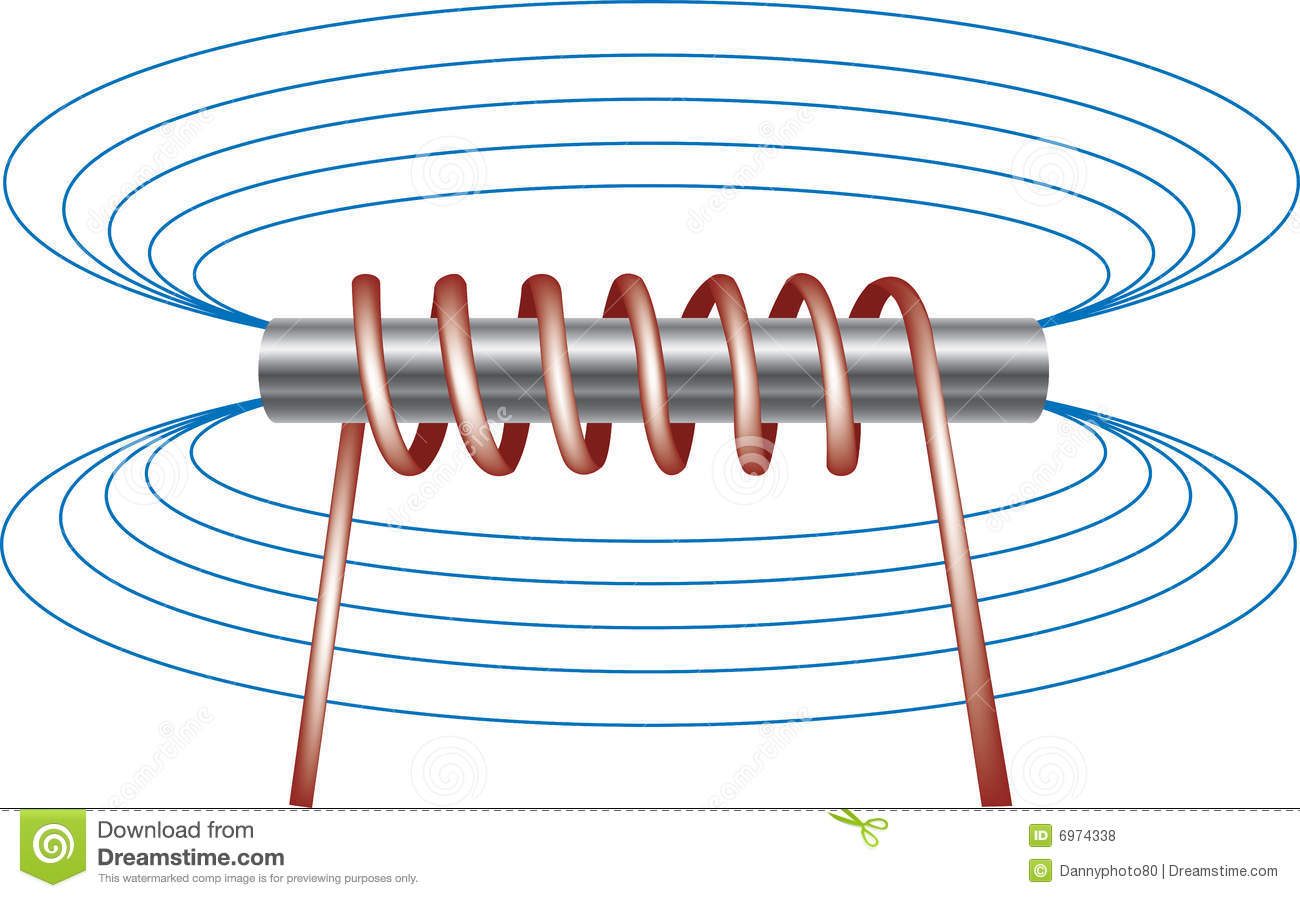
\includegraphics[scale=0.65]{src/images/Solenoide.jpg}
\caption{Bobina de tipo solenoide}
\label{fgr:Solenoide}
\end{figure}

\begin{figure}[H]
\centering
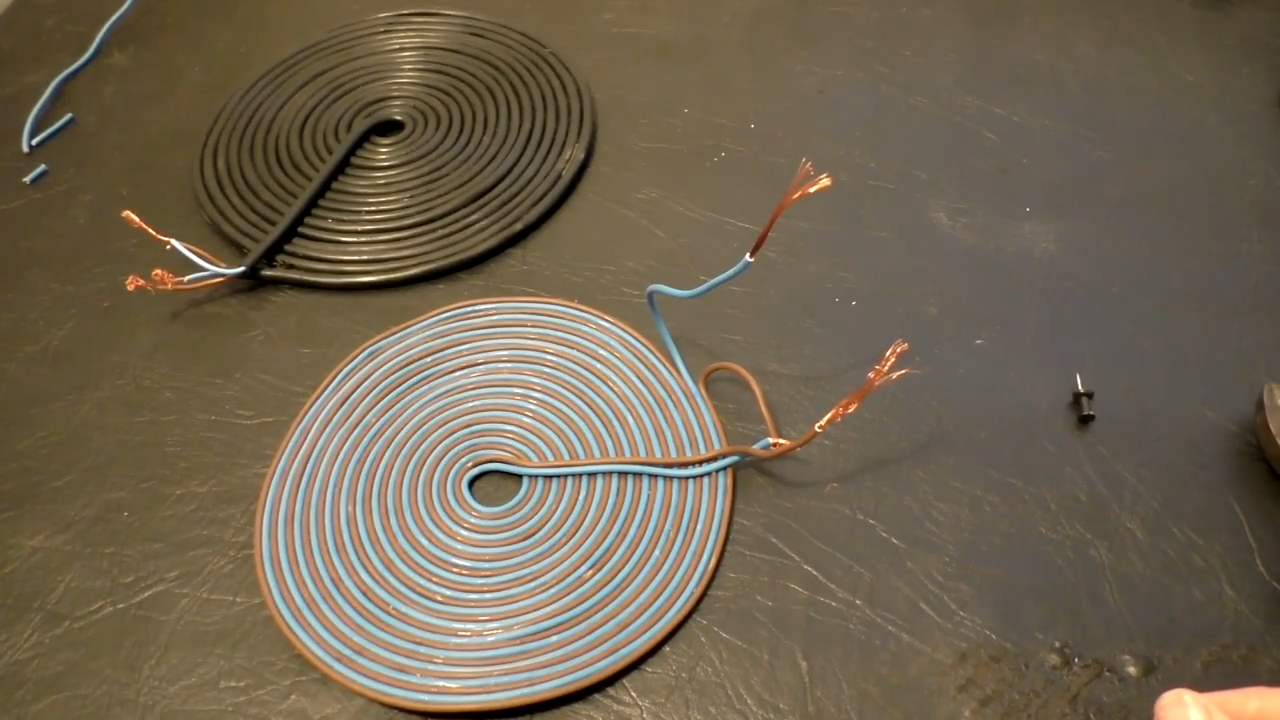
\includegraphics[scale=0.3]{src/images/Pancake.png}
\caption{Bobina de tipo pancake}
\label{fgr:Pancake}
\end{figure}

\subsubsection{Transformador}
El transformador es un dispositivo que permite modificar potencia eléctrica de corriente alterna con un determinado valor de tensión y corriente en otra potencia de casi el mismo valor pero, generalmente con distintos valores de tensión y corriente.

Es una máquina estática de bajas pérdidas y tiene un uso muy extendido en los sistemas eléctricos de transmisión y distribución de energía eléctrica.

\begin{figure}[H]
\centering
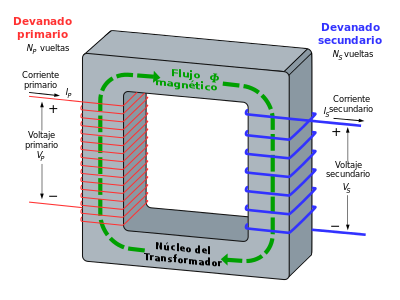
\includegraphics[scale=0.75]{src/images/Transformador.png}
\caption{Transformador monofásico de núcleo de hierro}
\label{fgr:Transformador}
\end{figure}

\subsubsection{Perdidas de un transformador}
Las pérdidas de potencia en un transformador real, son un tema muy crítico y complicado, dichas pérdidas han sido estudiadas por años y años, llegando a la conclusión de que es imposible no tener pérdidas en un transformador; es por esto que ahora lo que se pretende lograr es reducir las pérdidas lo máximo posible.

Un transformador real tiene perdidas por diferentes circunstancias, no solo por una, y sin embargo todas se manifiestan en forma de calor, es decir si un transformador tiene pérdida de potencia esta pérdida se transformara en calor, este es el principio de la conservación de energía.

Con el fin de tratar de reducir las pérdidas de potencia lo máximo posible, sea estudiado cuales son las causas por las que se producen estas pérdidas y así hacer algo al respecto y tomar una medida adecuada y oportuna que permita una solución al problema; esta solución claramente no será una solución totalmente exitoso pero lograra una mejora muy considerable. \\

Las perdidas en un transformador son las siguientes:

\begin{enumerate}
\item Flujos dispersos
\item Ciclo de histeresis
\item Corrientes parasitas
\item Perdidas en los bobinados
\end{enumerate}

\subsection{Componentes electrónicos}

\section{Desarrollo del proyecto}

\subsection{Diseño de los circuitos}
Nuestro objetivo para lograr el calentamiendo del material que deseemos es, como podemos deducir de lo visto anteriormente, al aumentar las perdidas en el nucleo por corrientes paracitas y corrientes de Folcaut, reducir al minimo las del bobinado por efecto Joule y flujo disperso, se lograra una alta eficiencia en nuestro calentador.

\subsubsection{Oscilador de alta frecuencia}
Para aumentar las perdidas por corrientes de Folcaut en el ferromágnetico debemos aumentar la frecuencia de oscilacion del primario. \\

Para ello, lo mas sencillo es optar por un oscilador RLC, configurado de tal forma que oscile a una frecuencia superior a los 10kHz. Lo que producira gran cantidad de perdidas.

\begin{figure}[H]
\centering
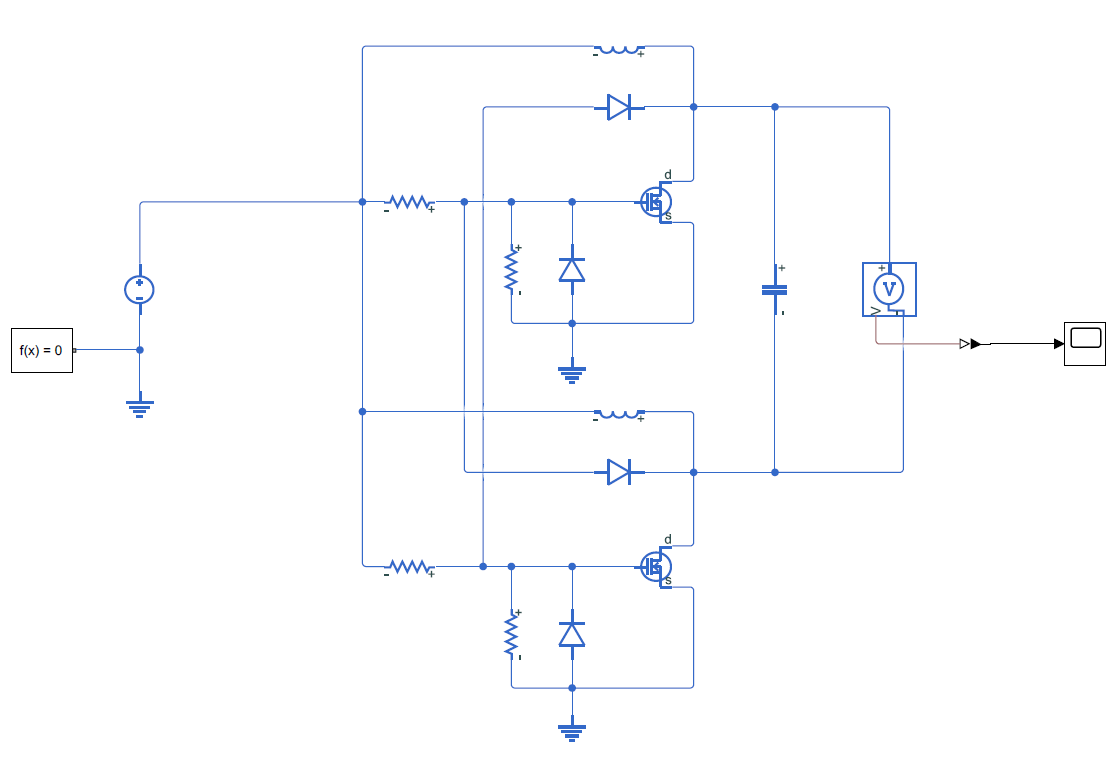
\includegraphics[scale=0.75]{src/images/Oscilador.png}
\caption{Esquemático de un oscilador senoidal}
\label{fgr:Oscilador}
\end{figure}

En la Figura \eqref{fgr:Oscilador} se puede observar el circuito que generará la siguiente salida la cual se conectará a una bobina para producir el campo mágnetico.

\begin{figure}[H]
\centering
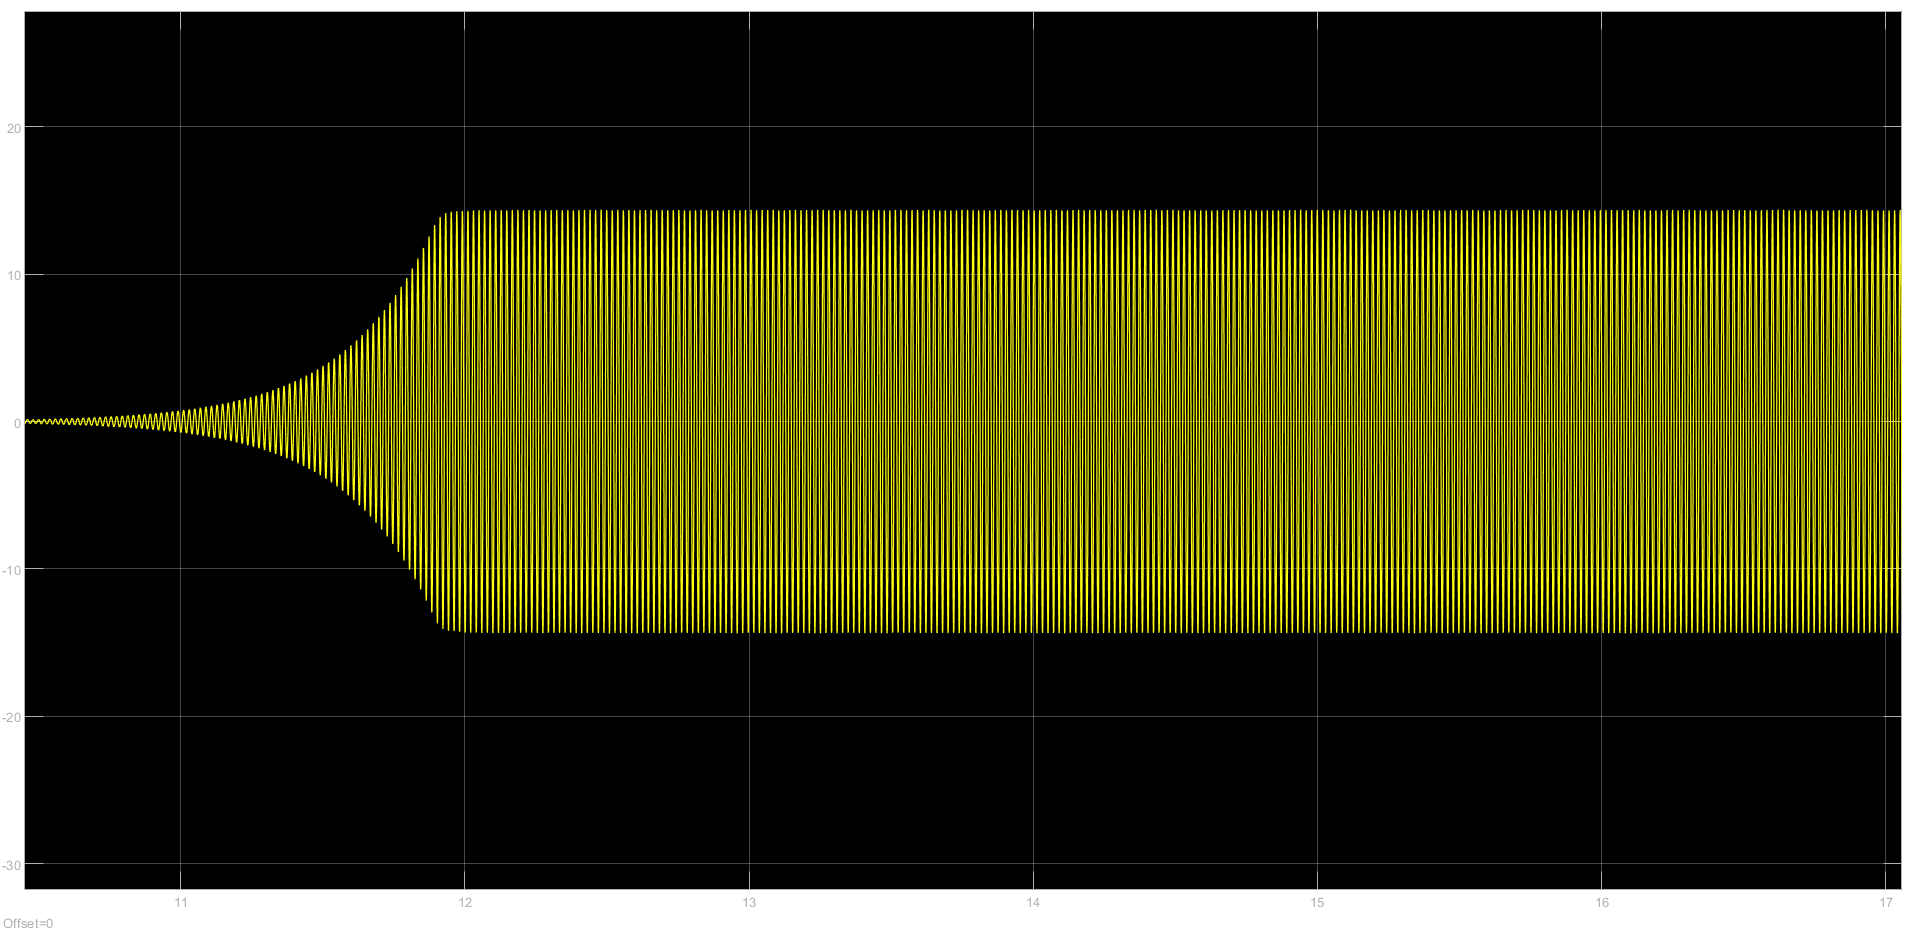
\includegraphics[scale=0.3]{src/images/Onda_larga.png}
\caption{Forma de onda de salida a la bobina en periodo muy largo}
\label{fgr:Onda_super_larga}
\end{figure}

\begin{figure}[H]
\centering
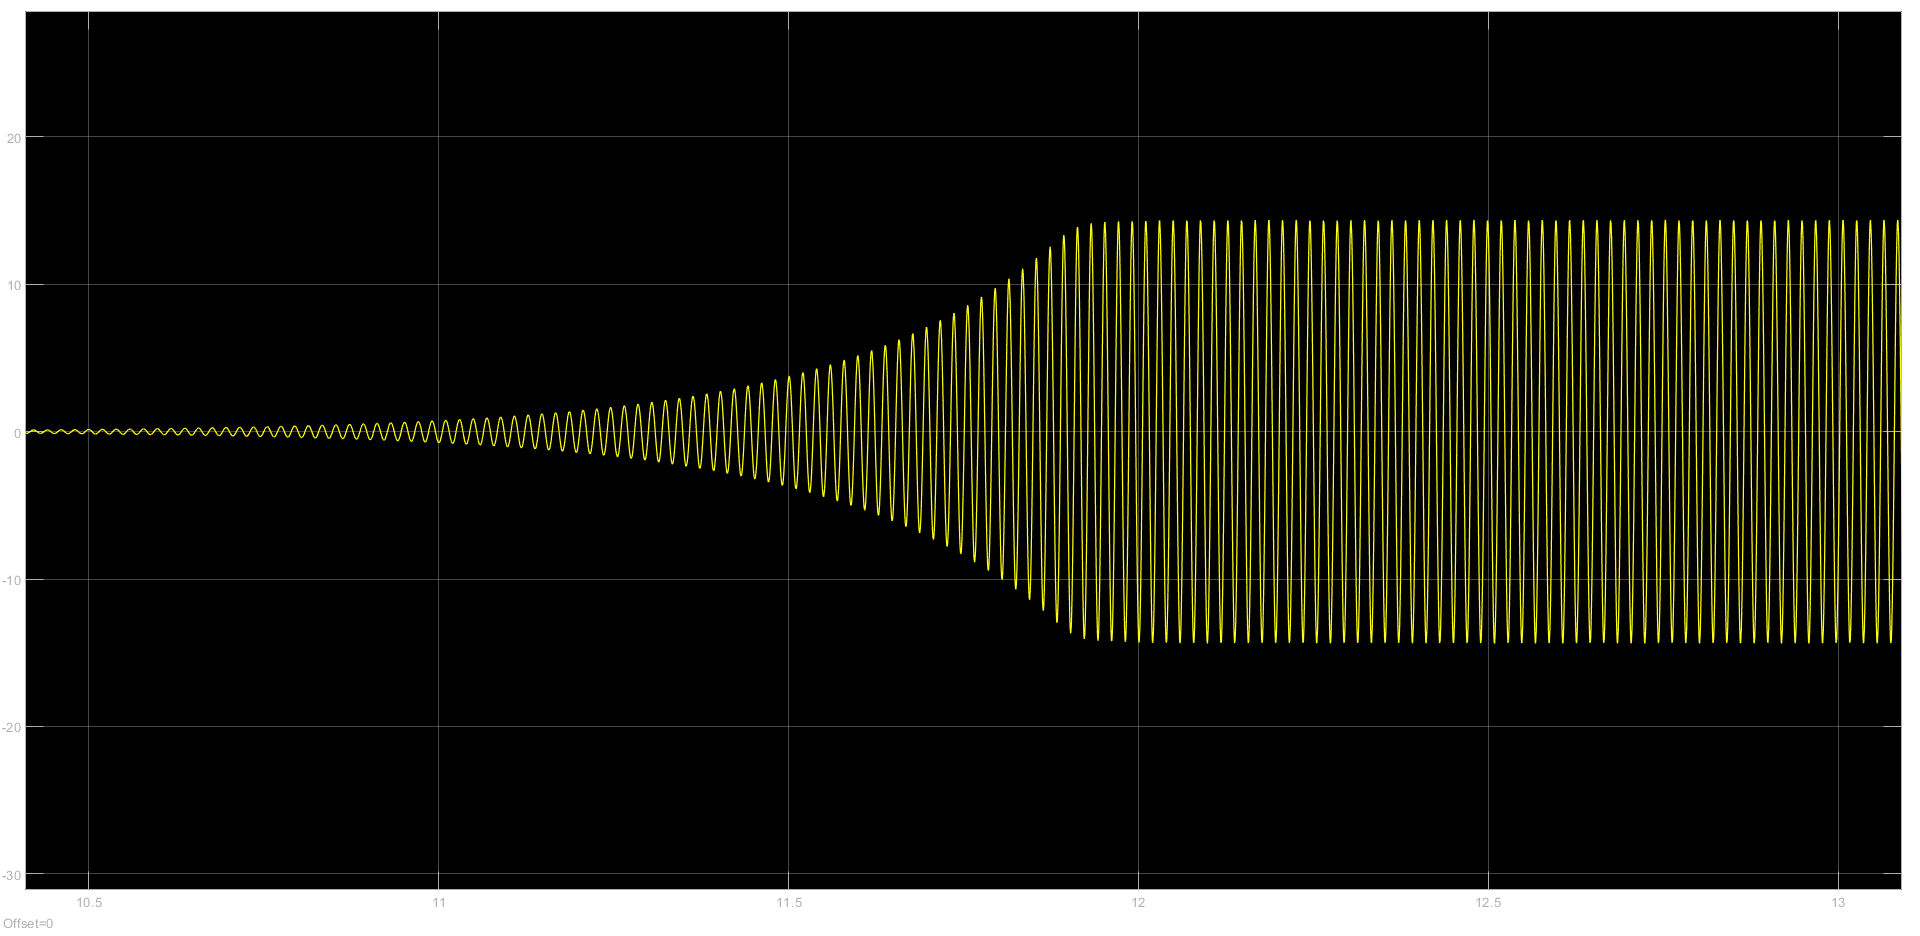
\includegraphics[scale=0.3]{src/images/Onda_corta.png}
\caption{Forma de onda de salida a la bobina en periodo largo}
\label{fgr:Onda_larga}
\end{figure}

\begin{figure}[H]
\centering
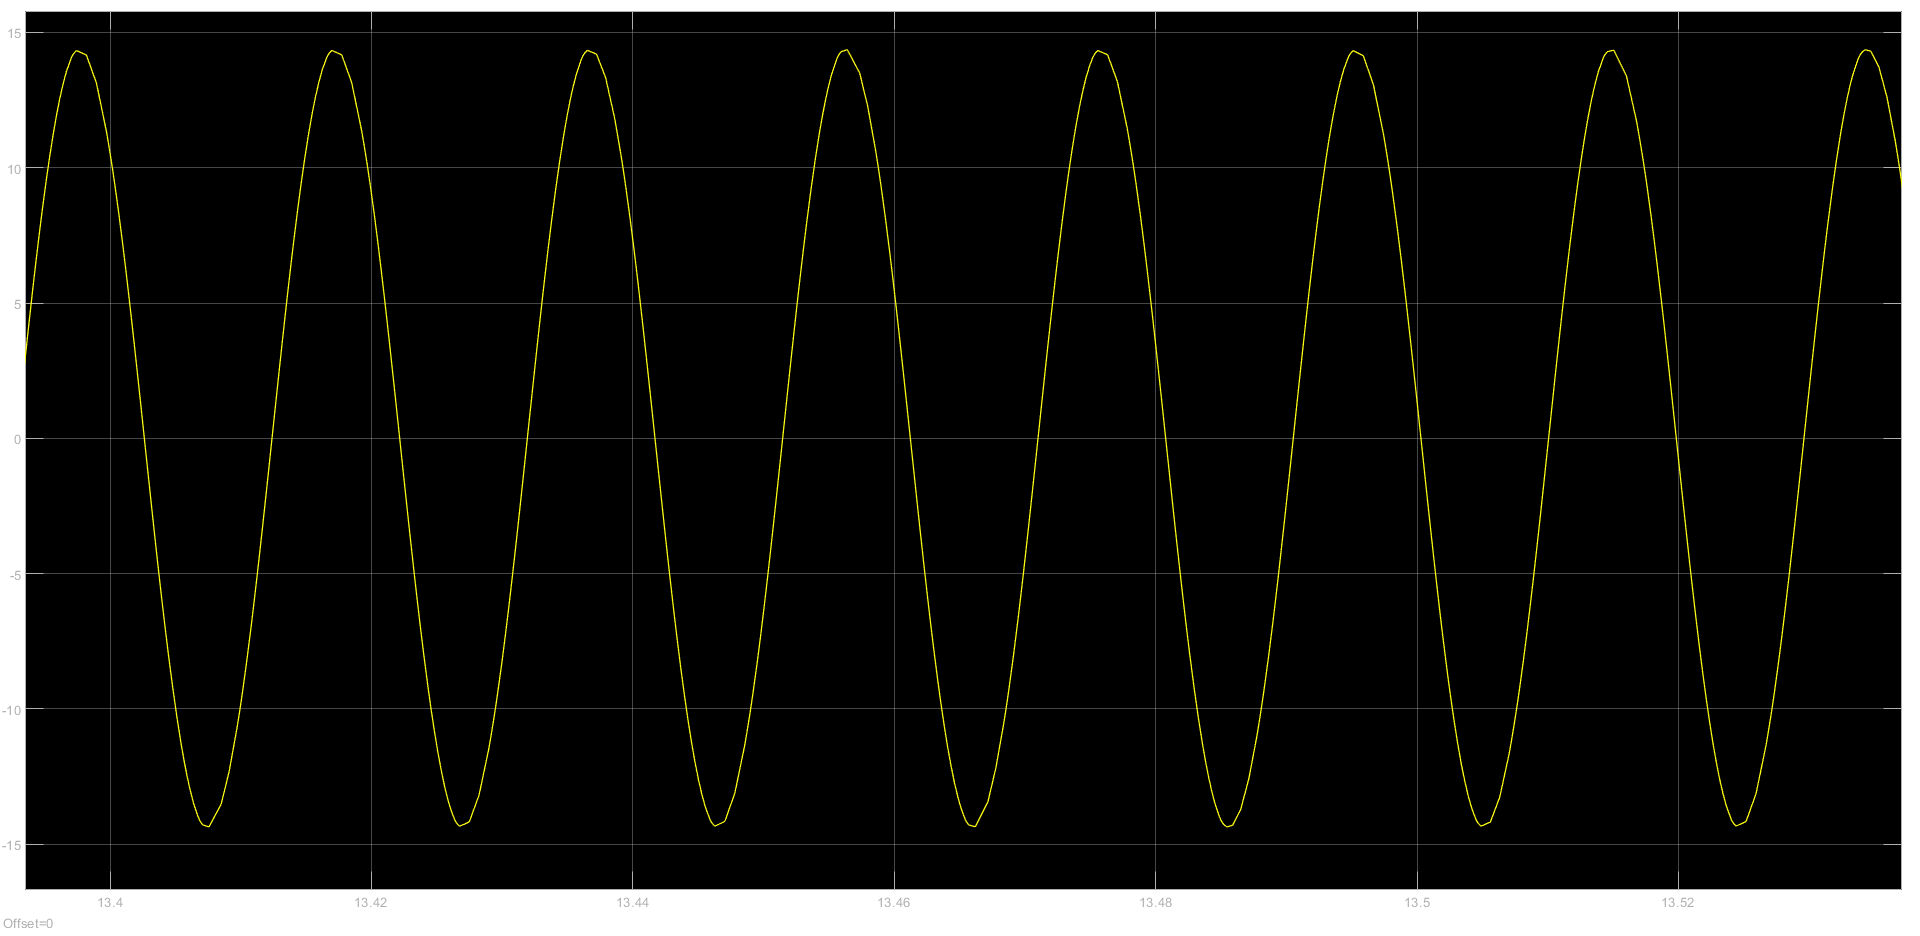
\includegraphics[scale=0.3]{src/images/Onda_muy_corta.png}
\caption{Forma de onda de salida a la bobina en periodo corto}
\label{fgr:Onda_corta}
\end{figure}

% Referencias bibliograficas
\newpage

\begin{thebibliography}{99}
\bibitem{Libro 1} ROBERT L.BOYLESTAD Y LOUIS NASHELSKY. Electrónica: teoría de circuitos y dispositivos electrónicos, décima edición.
\end{thebibliography}

\end{document}